\section{Network Training}
\label{sec:network-training}

Network training describes the problem of determining the parameters to model the target function. Therefore, we use a set of training data representing the initial knowledge of the target function. Often the target function is unknown and we only know the value of the function for specific data points.

Depending on the training set we consider three different learning paradigms \cite[p.~85-88]{Haykin:2005}:
\begin{description}
\item[Unsupervised learning] The training set provides only input values. The neural network has to find similarities by itself.
\item[Reinforcement learning] After processing an input value of the training set the neural network gets feedback whether the result is considered good or bad.
\item[Supervised learning] The training set provides both input values and desired target values (labeled training set).
\end{description}

Although the human brain mostly learns by reinforcement learning (or even unsupervised learning), we discuss supervised learning only. Let $T := \{(x_n, t_n) : 1 \leq n \leq N\}$ be a training set where $x_n$ are input values and $t_n$ the corresponding target values. As for any approximation problem we can evaluate the performance of the neural network using some distance measure between approximation and target function.

\subsection{Error Measures}
\label{subsec:error-measures}

We discuss mainly two error measures. The sum-of-squared error function takes the form
\begin{align}
E (w) = \sum _{n = 1} ^N E_n (w) = \frac{1}{2} \sum _{n = 1} ^N \sum _{k = 1} ^C (y_k(x_n,w) - t_{nk})^2
\end{align}
where $t_{nk}$ denotes the $k^{\text{th}}$ entry of the $n^{\text{th}}$ target value. The cross-entropy error function is given by
\begin{align}
E(w) = \sum _{n = 1} ^N E_n (w) = - \sum _{n = 1} ^N \sum _{k = 1} ^C t_{nk} \log(y_k(x_n, w))\onedot
\end{align}

For further discussion we note that by using $y_i(x_n,w) = f (z_i)$ the derivatives of both error functions with respect to the actual input $z_i^{(L+1)}$ of the $i^{\text{th}}$ output unit take the form
\begin{align}
\frac{\partial E_n}{\partial z_i^{(L+1)}} = \frac{\partial E_n}{\partial y_i^{(L+1)}} \frac{\partial y_i^{(L+1)}}{\partial z_i^{(L+1)}} = y_i(x_n,w) - t_{ni}\onedot
\end{align}
Here we use the softmax activation function for the cross-entropy error function and the identity as activation function for the sum-of-squared error function \cite[p.~230-231,236-240]{Bishop:1995}.

\subsection{Training Approaches}

Given an error function $E(w) = \sum _{n = 1} ^N E_n (w)$ we distinguish mainly two different training approaches \cite[p.~293-295]{DudaHartStork:2001}:
\begin{description}
\item[Stochastic training] Randomly choose an input value $x_n$ and propagate it through the network. Update the weights based on the error $E_n(w)$.
\item[Batch training] Go through all input values $x_n$ and compute $y(x_n,w)$. Update the weights based on the overall error $E(w) = \sum _{n = 1} ^N E_n(w)$.
\end{description}
Instead of choosing an input value $x_n$ at random we could also select the input values in sequence leading to sequential training. As of \cite[p.~240-241]{Bishop:2006} stochastic training is considered to be faster especially on redundant training sets.

\subsection{Parameter Optimization}
\label{subsec:parameter-optimization}

The weight update in both approaches is determined by a parameter optimization algorithm which tries to minimize the error. The error $E(w)$ can be considered as error surface above the weight space. In general, the error surface is a nonlinear function of the weights and may have many local minima and maxima. We want to find the global minimum. The necessary criterion to find a minimum is
\begin{align}
\nabla E (w) = 0
\end{align}
where $\nabla E$ denotes the gradient of the error function $E$ evaluated at point $w$.

As an analytical solution is usually not possible we use an iterative approach for minimizing the error. In each iteration step we choose an weight update $\Delta w[t]$ and set
\begin{align}
w[t + 1] = w[t] + \Delta w[t]
\end{align}
where $w[t]$ denotes the weight vector $w$ in the $t^{\text{th}}$ iteration and $w[0]$ is an appropriate starting vector. Optimization algorithms differ in choosing the weight update $\Delta w[t]$ \cite[p.~254-256]{Bishop:1995}. Before discussing two common optimization algorithms, we discuss the case of linear units and the problem of choosing a good starting vector $w[0]$.

\subsubsection{Linear Units}

In the case of a single-layer perceptron with linear output units and sum-of-squared error we obtain a linear problem. Thus, we can determine the weights exactly using singular value decomposition \cite[p.~259-260]{Bishop:1995}.

When considering a multilayer perceptron with linear output units and nonlinear hidden units we can at least split up the problem of minimization. The weights in the output layer can be determined exactly using singular value decomposition whereas the weights in the hidden layers can be optimized using an iterative approach. Note that every time the weights of the nonlinear layers are updated the exact solution for the weights in the output layer has to be recomputed \cite[p.~259-260]{Bishop:1995}.

\subsubsection{Weight Initialization}

Following \cite[p.~311-312]{DudaHartStork:2001} we want to get a starting vector $w$ such that we have fast and uniform learning, that is all components learn more or less equally fast. Assuming sigmoidal activation functions the actual input of a unit should neither be too large causing $\sigma'(z)$ to be very small nor be too small such that $\sigma(z)$ is approximately linear. Both cases will result in slow learning. For the logistic sigmoid an acceptable value for the unit input is of unity order \cite[p.~260-262]{Bishop:1995}. Thus, we choose all weights randomly from the same distribution such that
\begin{align}
- \frac{1}{\sqrt{m^{(l - 1)}}} < w_{ij}^{(l)} < \frac{1}{\sqrt{m^{(l - 1)}}}
\end{align}
for the weights in layer $l$. Assuming a normal distribution with zero mean and unity variance for the inputs of each unit we get on average the desired actual input of unity order \cite[p.~311-312]{DudaHartStork:2001}.

\subsubsection{Gradient Descent}

Gradient descent is a basic first-order optimization algorithm. This means that in every iteration step we use information about the gradient $\nabla E$ at the current point. In iteration step $[t + 1]$ the weight update $\Delta w[t]$ is determined by taking a step into the direction of the negative gradient at position $w[t]$ such that
\begin{align}
\Delta w[t] = - \gamma \frac{\partial E}{\partial w[t]}
\end{align}
where $\gamma$ is called learning rate. Gradient descent can be used both for batch training and stochastic training\cite[p.~240-241]{Bishop:2006}. In the case of stochastic training we choose
\begin{align}
\Delta w[t] = - \gamma \frac{\partial E_n}{\partial w[t]}
\end{align}
as weight update.

\subsubsection{Momentum}

\begin{figure}[t!]
	\centering
	\subfigure[High learning rate.]{
    		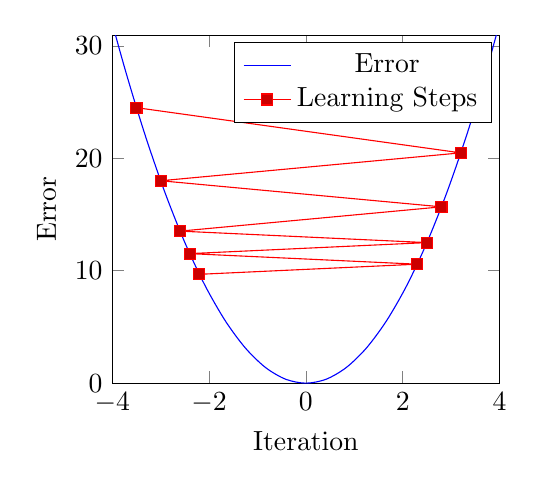
\begin{tikzpicture}
			\begin{axis}[height=6cm,width=6.5cm,ylabel=Error,xlabel=Iteration,xmin=-4,xmax=4,ymin=0]
				\addplot[blue,smooth] {2*x^2};
				\addlegendentry{Error}
				\addplot+[red] coordinates{(-3.5,24.5)(3.2,20.48)(-3,18)(2.8,15.68)(-2.6,13.52)(2.5,12.5)(-2.4,11.52)(2.3,10.58)(-2.2,9.68)};
				\addlegendentry{Learning Steps}
			\end{axis}
		\end{tikzpicture}
		\label{subfig:momentum-high}
	}
	\subfigure[Low learning rate.]{
		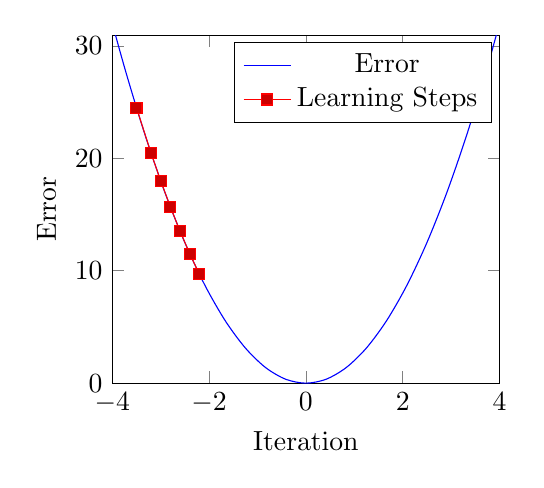
\begin{tikzpicture}
			\begin{axis}[height=6cm,width=6.5cm,ylabel=Error,xlabel=Iteration,xmin=-4,xmax=4,ymin=0]
				\addplot[blue,smooth] {2*x^2};
				\addlegendentry{Error}
				\addplot+[red] coordinates{(-3.5,24.5)(-3.2,20.48)(-3,18)(-2.8,15.68)(-2.6,13.52)(-2.4,11.52)(-2.2,9.68)};
				\addlegendentry{Learning Steps}
			\end{axis}
		\end{tikzpicture}
		\label{subfig:momentum-low}
	}
    	\caption[The learning rate and its influence on the rate of convergence.]{When using a large learning rate the weight updates in each iteration tend to overstep the minimum. This causes oscillation around the minimum. This observation is illustrated by figure \ref{subfig:momentum-high}. Choosing the learning rate too low will result in a slow convergence to the minimum as shown in figure \ref{subfig:momentum-low}. Both scenarios are visualized using a quadratic function we seek to minimize.}
    	\label{fig:momentum}
\end{figure}
The choice of the learning rate can be crucial. We want to choose the learning rate such that we have fast learning but avoid oscillation when choosing the learning rate too large \cite[p.~267-268]{Bishop:1995}. Both cases are illustrated by figure \ref{fig:momentum} where we seek to minimize a convex quadratic function. One way to reduce oscillation while using a high learning rate as described in \cite[p.~267-268]{Bishop:1995} is to add a momentum term. Then the change in weight is dependent on the previous change in weight such that
\begin{align}
\Delta w[t] = - \gamma \frac{\partial E}{\partial w[t]} + \lambda \Delta w[t - 1]
\end{align}
where $\lambda$ is called momentum parameter. %Evidently $\lambda$ should lie in the range $0 \leq \lambda \leq 1$.

\subsubsection{Enhanced Gradient Descent}

There is still a serious problem with gradient descent: how to choose the learning rate (and the momentum parameter). Currently, we are required to choose the parameters manually. Because the optimal values are dependent on the given problem, an automatic choice is not possible.

We discuss a simple approach on choosing the learning rate automatically considering no momentum term. Let $\gamma [t]$ denote the learning rate in the $t^{\text{th}}$ iteration. Then we have a simple criterion on whether the learning rate was chosen too large: If the error has increased after the weight update we may have overstepped the minimum. Then we can undo the weight update and choose a smaller learning rate until the error decreases \cite[p.~268-272]{Bishop:1995}. Thus, we have
\begin{align}
\gamma [t + 1] = 
\begin{cases}
\rho \cdot \gamma [t] & \text{if } E(w[t + 1]) < E(w[t]) \\
\mu \cdot \gamma [t] & \text{if } E(w[t + 1]) > E(w[t])
\end{cases}
\end{align}
where the update parameters can be chosen as suggested in \cite[p.~268-272]{Bishop:1995}: set $\rho := 1.1$ to avoid frequent overstepping of the minimum; set $\mu := 0.5$ to ensure fast recovery to taking a step which minimizes the error.

% \subsubsection{Second Order Methods}
%
% Although gradient descent has been improved in many ways it is considered a poor optimization algorithm as pointed out in \cite[p.~268-269]{Bishop:1995} and \cite[p.~240-241]{Bishop:2006}. But optimization is a widely studied area and, thus, there are more efficient algorithms. Conjugate gradients makes implicit use of second order information. Newton's Method or so called Quasi-Newton Methods explicitly use the Hessian of the error function in each iteration step. Some of these algorithms are described in detail in \cite[p.~274-290]{Bishop:1995}.

\subsubsection{Newton's Method}

Although gradient descent has been improved in many ways it is considered a poor optimization algorithm as pointed out in \cite[p.~268-269]{Bishop:1995} and \cite[p.~240-241]{Bishop:2006}. But optimization is a widely studied area and, thus, there are more efficient algorithms. Conjugate gradients makes implicit use of second order information. Newton's method or so called quasi-Newton methods explicitly use the Hessian of the error function in each iteration step. Some of these algorithms are described in detail in \cite[p.~274-290]{GillMurrayWright:1997}. We discuss the general idea of Newton's method.

Newton's method is an iterative optimization algorithm based on a quadratic approximation of $E$ using the Taylor series. Let $H(w[t])$ denote the Hessian of the error function evaluated at $w[t]$. Then, by taking the first three terms of the Taylor series\footnote{In general, the Taylor series of a smooth function $f$ at point $x_0$ is given by \begin{align}T(x) = \sum _{k = 0} ^\infty \frac{f^{(k)} (x_0)}{k!} (x - x_0)^k\onedot\end{align}}, we obtain a quadratic approximation of $E$ around the point~$w[t]$ \cite[p.~105-106]{GillMurrayWright:1997}:
\begin{align}
\tilde{E}(w[t] + \Delta w[t]) & = E(w[t]) + \nabla E(w[t])^{tr} \Delta w[t] + \frac{1}{2} (\Delta w[t])^{tr} H(w[t]) \Delta w[t]\onedot
\end{align}
We want to choose the weight update $\Delta w[t]$ such that the quadratic approximation $\tilde{E}$ is minimized. Therefore, the necessary criterion gives us:
\begin{align}
\nabla \tilde{E}(w[t] + \Delta w[t]) & = \nabla E(w[t]) + H(w[t]) \Delta w[t] \overset{!}{=} 0\onedot
\end{align}
The solution is given by
\begin{align}
\label{eq:newton-update}
\Delta w[t] = - \gamma H(w[t])^{-1} \nabla E(w[t])
\end{align}
where $H(w[t])^{-1}$ is the inverse of the Hessian at point $w[t]$. Because we use a quadratic approximation, equation \eqref{eq:newton-update} needs to be applied iteratively. When choosing $w[0]$ sufficiently close to the global minimum of $E$, Newton's method converges quadratically \cite[p.~105-106]{GillMurrayWright:1997}.

Nevertheless, Newton's method has several drawbacks. As we see later, the evaluation of the Hessian matrix and its inversion is rather expensive\footnote{The inversion of a $n \times n$ matrix usually requires $\mathcal{O}(n^3)$ operations.}. In addition, the Newton step in equation \eqref{eq:newton-update} may be a step in the direction of a local maximum or saddle point. This may happen if the Hessian matrix is not positive definite \cite[p.~285-287]{Bishop:1995}.

\subsection{Error Backpropagation}
\label{subsec:error-backpropagation}

Error backpropagation describes an efficient algorithm to evaluate $\nabla E_n$ for multilayer perceptrons using differentiable activation functions.

Following \cite[p.~241-245]{Bishop:2006} we consider the $i^\text{th}$ output unit first. The derivative of an arbitrary error function $E_n$ with respect to the weight $w_{ij}^{(L+1)}$ is given by
\begin{align}
\label{eq:partial-factors}
\frac{\partial E_n}{\partial w_{ij}^{(L+1)}} \underset{rule}{\overset{\text{chain-}}{=}} \frac{\partial E_n}{\partial z_i^{(L+1)}} \frac{\partial z_i^{(L+1)}}{\partial w_{ij}^{(L+1)}}
\end{align}
where $z_i^{(L+1)}$ denotes the actual input of the $i^\text{th}$ unit within the output layer. Using the chain rule, the first factor in equation \eqref{eq:partial-factors} can be written as
\begin{align}
\label{eq:output-first-factor}
\delta _i ^{(L+1)} := \frac{\partial E_n}{\partial z_i^{(L+1)}} & \underset{rule}{\overset{\text{chain-}}{=}} \frac{\partial E_n}{\partial y_i^{(L+1)}} \frac{\partial y_i^{(L+1)}}{\partial z_i^{(L+1)}}\notag\\
& = \frac{\partial E_n}{\partial y_i^{(L+1)}} f'\left(z_i^{(L+1)}\right)
\end{align}
where $\delta _i ^{(L+1)}$ is often called error and describes the influence of the $i^\text{th}$ output unit on the total error $E_n$. The second factor of equation \eqref{eq:partial-factors} takes the form
\begin{align}
\label{eq:output-second-factor}
\frac{\partial z_i^{(L+1)}}{\partial w_{ij}^{(L+1)}}
& = \frac{\partial}{\partial w_{ij}^{(L+1)}} \left[\sum _{k = 0} ^{m^{(L)}} w_{ik}^{(L+1)}y_k^{(L)}\right]\notag\\
& = \frac{\partial}{\partial w_{ij} ^{(L+1)}} \left[w_{ij}^{(L+1)}y_j^{(L+1)} + \underbrace{\sum _{k = 0, k \neq i} ^{m^{(L)}} w_{ik}^{(L+1)} y_k^{(L)}}_{const.}\right]\notag\\
& =  y_j^{(L)}\onedot
\end{align}
By substituting both factors \eqref{eq:output-first-factor} and \eqref{eq:output-second-factor} into equation \eqref{eq:partial-factors} we get
\begin{align}
\label{eq:derivative}
\frac{\partial E_n}{\partial w_{ij}^{(L+1)}} = \delta _i^{(L+1)} y_j^{(L)}\onedot
\end{align}
The errors $\delta_i ^{(L+1)}$ are usually easy to compute, for example when choosing error function and output activation function as noted in section \ref{subsec:error-measures}.

\begin{SCfigure}[2\sidecaptionrelwidth][t!]
	\centering
	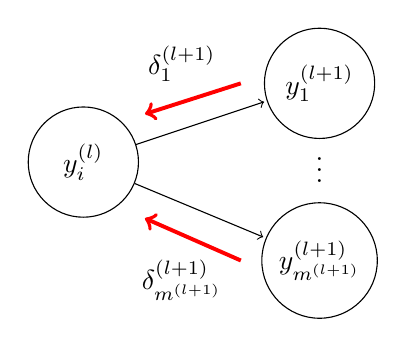
\begin{tikzpicture}[shorten >=1pt]
      		\tikzstyle{unit}=[draw,shape=circle,minimum size =1.4cm]

       	\node[unit](i) at (0,1){$y_i^{(l)}$};
        	\node[unit](k1) at (3,2){$y_1^{(l+1)}$};
		\node at (3, 1){$\vdots$};
		\node[unit](km) at (3,-0.25){$y_{m^{(l+1)}}^{(l+1)}$};
		
		\node at (1.25,2.25){$\delta_1^{(l+1)}$};
		\node at (1.25,-0.5){$\delta_{m^{(l+1)}}^{(l+1)}$};

        	\draw[->] (i) -- (k1);
		\draw[->] (i) -- (km);
		
		\draw[->,red,line width=0.05cm] (2,-0.25) -- (0.75,0.3);
		\draw[->,red,line width=0.05cm] (2,2) -- (0.75,1.6);
    	\end{tikzpicture}
	\caption[Backpropagation of errors through the network.]{Once evaluated for all output units, the errors $\delta_i^{(L+1)}$ can be propagated backwards according to equation~\eqref{eq:hidden-delta}. The derivatives of all weights in layer $l$ can then be determined using equation~\eqref{eq:derivative}.}.
	\label{fig:error-backpropagation}
\end{SCfigure}

Considering the $i^\text{th}$ hidden unit within an arbitrary hidden layer $l$ we write
\begin{align}
\label{eq:evaluate-derivative}
\frac{\partial E_n}{\partial w_{ij}^{(l)}} \underset{rule}{\overset{\text{chain-}}{=}} \frac{\partial E_n}{\partial z_i^{(l)}} \frac{\partial z_i^{(l)}}{\partial w_{ij}^{(l)}}
\end{align}
and notice that the second factor in equation \eqref{eq:evaluate-derivative} takes the same form as in equation \eqref{eq:output-second-factor}:
\begin{align}
\frac{\partial z_i^{(l)}}{\partial w_{ij}^{(l)}} = \frac{\partial}{\partial w_{ij}^{(l)}} \left[\sum _{k = 0} ^{m^{(l-1)}} w_{ik}^{(l)}y_k^{(l-1)}\right] = y_j^{(l-1)}\onedot
\end{align}
Thus, only the error $\delta _i ^{(l)}$ changes. Using the chain rule we get
\begin{align}
\label{eq:hidden-delta}
\delta _i ^{(l)} := \frac{\partial E_n}{\partial z_i^{(l)}} = \sum _{k = 1} ^{m^{(l+1)}} \frac{\partial E_n}{\partial z_k^{(l+1)}} \frac{\partial z_k^{(l+1)}}{\partial z_i^{(l)}}\onedot
\end{align}
In general, the sum runs over all units directly succeeding the $i^\text{th}$ unit in layer $l$ \cite[p.~242-245]{Bishop:2006}. But we assume that every unit in layer $l$ is connected to every unit in layer $(l+1)$ where we allow the weights $w_{ki}^{(l+1)}$ to vanish. Altogether, by substituting the definition of $\delta _k ^{(l+1)}$ from equation \eqref{eq:hidden-delta} we have
\begin{align}
\label{eq:delta-backpropagation}
\delta _i ^{(l)} = f' \left(z_i^{(l)}\right) \sum _{k = 1} ^{m^{(l+1)}} w_{ik}^{(l+1)} \delta _k ^{(l+1)}\onedot
\end{align}

In conclusion, we have found a recursive algorithm for calculating the gradient $\nabla E_n$ by propagating the errors $\delta _i ^{(L+1)}$ back through the network using equation \eqref{eq:delta-backpropagation} and evaluating the derivatives $\frac{\partial E_n}{\partial w_{ij}^{(l)}}$ using equation \eqref{eq:evaluate-derivative}.

%\begin{Alg}[Error Backpropagation]
%\begin{enumerate}[1.]
%\item Propagate the input value $x_n$ through the network to get the actual input and output of all units.
%\item Calculate $\delta _j ^{(L+1)}$ for all output units and determine $\delta _j ^{(l)}$ for all hidden layers $l$ by using backpropagation:
%\begin{align}
%\label{eq:delta-hidden}
%\delta _j ^{(l)} = f' (z_j^{(l)}) \sum _{k = 1} ^{m^{(l+1)}} w_{ik}^{(l+1)} \delta _k ^{(l+1)}
%\end{align}
%\item Calculate the required derivatives:
%\begin{align}
%\frac{\partial E_n}{\partial w_{ji}^{(l)}} = \delta _j ^{(l)} y_i^{(l-1)}
%\end{align}
%\end{enumerate}
%\end{Alg}

\subsubsection{Efficiency}

The number of operations required for error backpropagation scales with the total number of weights $W$ and the number of units. Considering a sufficiently large multilayer perceptron such that every unit in layer $l$ is connected to every unit in layer $(l+1)$ the cost of propagating an input value through the network is dominated by $W$. Here we neglect the evaluation cost of the activation functions. Because of the weighted sum in equation~\eqref{eq:hidden-delta}, backpropagating the error is dominated by $W$, as well. This leads to an overall effort linear in the total number of weights: $\mathcal{O}(W)$ \cite[p.~246-247]{Bishop:2006}.

\subsection{The Hessian}

Following \cite{Bishop:1992} we derive an algorithm which allows us to evaluate the Hessian exactly by forward and backward propagation. Again, we assume differentiable activation functions within a multilayer perceptron. 

We start by picking two weights $w_{ij}^{(p)}$ and $w_{rs}^{(l)}$ where we assume the layer $p$ to come before layer $l$, that is $p \leq l$. The case where $p > l$ will follow by the symmetry of the Hessian \cite{Bishop:1992}. Figure \ref{fig:hessian} illustrates this setting for $p < (l - 1)$.
\begin{SCfigure}[\sidecaptionrelwidth][t!]
	\centering
	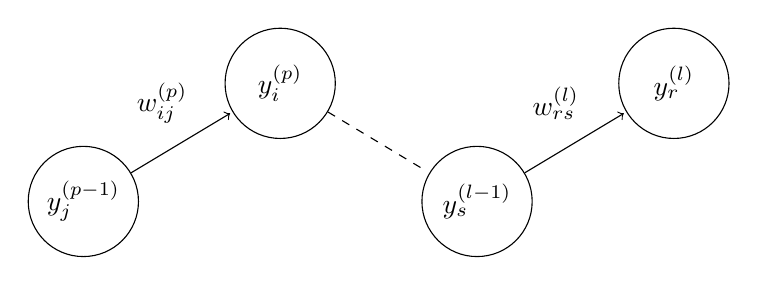
\begin{tikzpicture}[shorten >=1pt]
      		\tikzstyle{unit}=[draw,shape=circle,minimum size =1.4cm]

       	\node[unit](j) at (0,0){$y_j^{(p-1)}$};
        	\node[unit](i) at (2.5,1.5){$y_i^{(p)}$};

		\node[unit](s) at (5,0){$y_s^{(l-1)}$};
		\node[unit](r) at (7.5,1.5){$y_r^{(l)}$};
		
		\node at (1,1.25) {$w_{ij}^{(p)}$};
		\node at (6,1.25) {$w_{rs}^{(l)}$};
		
        	\draw[->] (j) -- (i);
        	\draw[dashed] (i) -- (s);
		\draw[->] (s) -- (r);
    	\end{tikzpicture}
	\caption[Exact evaluation of the Hessian.]{To derive an algorithm for evaluating the Hessian we consider two weights $w_{ij}^{(p)}$ and $w_{rs}^{(l)}$ where we assume that $p \leq l$. This figure illustrates the case when $p < (l - 1)$.}
	\label{fig:hessian}
\end{SCfigure}
As the error $E_n$ is only depending on $w_{ij}^{(p)}$ through the actual input $z_i^{(p)}$ of the $i^\text{th}$ unit in layer $p$ we start by writing
\begin{align}
\frac{\partial^2 E_n}{\partial w_{ij}^{(p)} \partial w_{rs}^{(l)}} \underset{rule}{\overset{\text{chain-}}{=}} \frac{\partial z_i^{(p)}}{\partial w_{ij}^{(p)}} \frac{\partial}{\partial z_i^{(p)}} \left(\frac{\partial E_n}{\partial w_{rs}^{(l)}}\right)\notag\\\overset{\eqref{eq:output-second-factor}}{=} y_j^{(p - 1)} \frac{\partial}{\partial z_i^{(p)}} \left(\frac{\partial E_n}{\partial w_{rs}^{(l)}}\right)\onedot
\end{align}
Now we remember the definition of $\delta _r ^{(l)}$ in equation \eqref{eq:hidden-delta} and add two more definitions:
\begin{align}
\label{eq:g-b}
g_{si} ^{(l - 1,p)} := \frac{\partial z_s^{(l - 1)}}{\partial z_i^{(p)}} \text{ and } b_{ri} ^{(l,p)} := \frac{\partial \delta_r ^{(l)}}{\partial z_i^{(p)}}\onedot
\end{align}
As $E_n$ is depending on $w_{rs}^{(l)}$ only through the value of $z_r^{(l)}$ we use the chain rule and write
\begin{align}
\frac{\partial^2 E_n}{\partial w_{ij}^{(p)} \partial w_{rs}^{(l)}} & = \frac{\partial}{\partial z_i^{(p)}} \left[y_j^{(p - 1)} \frac{\partial z_r^{(l)}}{\partial w_{rs}^{(l)}} \frac{\partial E_n}{\partial z_r^{(l)}}\right]\notag\\
 & = \frac{\partial}{\partial z_i^{(p)}} \left[y_j^{(p - 1)}   y_s^{(l-1)}\frac{\partial E_n}{\partial z_r^{(l)}}\right]\notag\\
 & \overset{\eqref{eq:hidden-delta}}{=} \frac{\partial}{\partial z_i^{(p)}} \left[y_j^{(p - 1)} y_s^{(l-1)}\delta_r^{(l)}\right]\onedot
\end{align}
Because the output $y_j^{(p-1)}$ of the $j^\text{th}$ unit in layer $(p - 1)$ is not depending on $z_i^{(p)}$, we can use the product rule and plug in the definitions from equation \eqref{eq:g-b}:
\begin{align}
\label{eq:hessian-evaluation}
\frac{\partial^2 E_n}{\partial w_{ij}^{(p)} \partial w_{rs}^{(l)}} & \underset{rule}{\overset{\text{product-}}{=}} y_j^{(p-1)} f'\left(z_s^{(l-1)}\right) \frac{\partial z_s^{(l-1)}}{\partial z_i^{(p)}} + y_j^{(p-1)} y_s^{(l-1)} \frac{\partial \delta _r ^{(l)}}{\partial z_i ^{(p)}}\notag\\
& \overset{\eqref{eq:g-b}}{=} y_j^{(p-1)} f'\left(z_s^{(l-1)}\right) g_{si}^{(l-1,p)} + y_j^{(p-1)} y_s^{(l-1)} b_{pi}^{(l,p)}\onedot
\end{align}

Following this derivation, Bishop suggests a simple algorithm to evaluate the $g_{si}^{(l-1,p)}$ and the $b_{ri}^{(l,p)}$ by forward and backward propagation. Using the chain rule we can write
\begin{align}
g_{si} ^{(l - 1,p)} \overset{\eqref{eq:g-b}}{=} \frac{\partial z_s^{(l - 1)}}{\partial z_i^{(p)}} & \underset{rule}{\overset{\text{chain-}}{=}} \sum _{k = 1} ^{m^{(l - 2)}} \frac{\partial z_s^{(l-1)}}{\partial z_k^{(l - 2)}} \frac{\partial z_k^{(l - 2)}}{\partial z_i^{(p)}}\notag\\
& = \sum _{k = 1} ^{m^{(l - 2)}} f'\left(z_k^{(l - 2)}\right) w_{sk}^{(l - 1)} g_{ki}^{(l-2)}\onedot
\end{align}
Initially we set $g_{ii}^{p,p} = 1$ and $g_{si}^{l,p} = 0$ for $l \leq p$. Thus, the $g_{si}^{(l-1,p)}$ can be obtained by forward propagating them through the network. Using the definition of $\delta_r^{(l)}$ from equation \eqref{eq:hidden-delta}, the product rule and the definitions from equation \eqref{eq:g-b} we write
\begin{align}
\label{eq:backpropagation-b}
b_{ri} ^{(l,p)} & \overset{\eqref{eq:g-b}}{=} \frac{\partial \delta_r ^{(l)}}{\partial z_i^{(p)}} \overset{\eqref{eq:hidden-delta}}{=} \frac{\partial f'\left(z_r^{(l)}\right) \left(\sum _{k = 1}^{m^{(l+1)}} w_{kr}^{(l+1)} \delta_k^{(l+1)}\right)}{\partial z_i^{(p)}}\notag\\
& \underset{rule}{\overset{\text{product-}}{=}} f''\left(z_r^{(l)}\right) \frac{\partial z_r^{(l)}}{\partial z_i^{(p)}} \left[ \sum _{k = 1}^{m^{(l+1)}} w_{kr}^{(l+1)} \delta _k^{(l+1)}\right] + f'\left(z_r^{(l)}\right) \left[\sum _{k = 1} ^{m^{(l+1)}} w_{kr}^{(l+1)} \frac{\partial \delta_k^{(l+1)}}{\partial z_i^{(p)}}\right]\notag\\
& \overset{\eqref{eq:g-b}}{=} f''\left(z_r^{(l)}\right) g_{ri}^{(l,p)} \left[ \sum _{k = 1}^{m^{(l+1)}} w_{kr}^{(l+1)} \delta _k^{(l+1)}\right] + f'\left(z_r^{(l)}\right) \left[\sum _{k = 1} ^{m^{(l+1)}} w_{kr}^{(l+1)} b_{ki}^{(l+1,p)}\right]\onedot
\end{align}
Using equation \eqref{eq:backpropagation-b} we can backpropagate the $b_{ri}^{(l,p)}$ after evaluating $b_{ki}^{(L+1,p)}$ for all output units $k$:
\begin{align}
b_{ki}^{(L+1,p)} & \overset{\eqref{eq:g-b}}{=} \frac{\partial \delta_k^{(L+1)}}{\partial z_i^{(p)}} \overset{\eqref{eq:hidden-delta}}{=} \frac{\partial \left(\frac{\partial E_n}{\partial z_k^{(L+1)}}\right)}{\partial z_i^{(p)}}\notag\\
& = \frac{\partial^2 E_n}{\partial^2 z_k^{(L+1)}} \frac{\partial z_k^{(L+1)}}{\partial z_i^{(p)}} = \frac{\partial^2 E_n}{\partial^2 z_k^{(L+1)}} g_{ki} ^{(L+1,p)}\notag\\
& = g_{ki}^{(L+1),p)} \left[f''\left(z_k^{(L+1)}\right) \frac{\partial E_n}{\partial y_k^{(L+1)}} + f'\left(z_k^{(L+1)}\right) \frac{\partial ^2 E_n}{\partial \left(y_k^{(L+1)}\right)^2}\right]\onedot
\end{align}
The errors $\delta_r^{(l)}$ can be evaluated as seen in section \ref{subsec:error-backpropagation} using error backpropagation.

Altogether, we are able to evaluate the Hessian of $E_n$ by forward propagating the $g_{si}^{(l-1,p)}$ and backward propagating the $b_{ri}^{(l,p)}$ as well as the errors $\delta_r^{(l)}$ \cite{Bishop:1992}.

% \subsubsection{Diagonal Approximation}
%
% For several reasons it may be of importance to efficiently evaluate an approximation of the hessian matrix. We discuss an diagonal approximation of the hessian matrix as it is used for regularization using the Optimal Brain Damage algorithm \cite{LeCunDenkerSolla:1990}. Therefore, using the chain rule we write:
%\begin{align}
%\frac{\partial^2 E_n}{\partial w_{ij^2}^{(l)}} & = \frac{\partial}{\partial w_{ij}^{(l)}} \left[ \frac{\partial E_n}{\partial y_i^{(l)}} \frac{\partial y_i^{(l)}}{\partial w_{ij}^{(l)}} \right]\notag\\
%& = \frac{\partial}{\partial w_{ij}^{(l)}} \left[ \frac{\partial E_n}{\partial y_i^{(l)}} f'\left(z_i^{(l)}\right) \frac{\partial z_i^{(l)}}{\partial w_{ij}^{(l)}} \right]\notag\\
%& = \frac{\partial^2 E_n}{\partial w_{ij}^{(l)} \partial y_i^{(l)}} f'\left(z_i^{(l)}\right) y_j^{(l-1)} + \frac{\partial E_n}{\partial y_j^{(l)}} f''\left(z_i^{(l)}\right)\left(y_j^{(l-1)}\right)^2\onedot
%\end{align}

\subsubsection{Efficiency}

We require one step of forward propagation and backward propagation per unit within the network. Again, assuming a sufficiently large network such that the number of weights $W$ dominates the network, the evaluation of equation \eqref{eq:hessian-evaluation} requires $\mathcal{O}(W^2)$ operations.

\subsection{Regularization}

Now we focus on the ability of generalization. We saw that theoretically a neural network with a sufficiently large number of hidden units can model every continuous target function. The ability of a network to generalize can be observed using unseen test data not used for training, usually called a validation set. If the trained approximation of the target function works well for the validation set the network is said to have good generalization capabilities \cite[p.~227-228]{Haykin:2005}. Overtraining of the network may result in over-fitting of the training set, that is the network memorizes the training set but performs very poorly on the validation set \cite[p.~227-228]{Haykin:2005}.

Regularization tries to avoid over-fitting and to give a better generalization performance. This can be achieved by controlling the complexity of the network which is mainly determined by the number of hidden units. The simplest form of regularization is adding a regulizer to the error function such that
\begin{align}
\hat{E}(w) = E(w) + \eta P(w)
\end{align}
where $P(w)$ is a penalty term which tries to influence the form and complexity of the solution \cite[p.~338]{Bishop:1995}.

\begin{SCfigure}[\sidecaptionrelwidth][t!]
	\centering
    	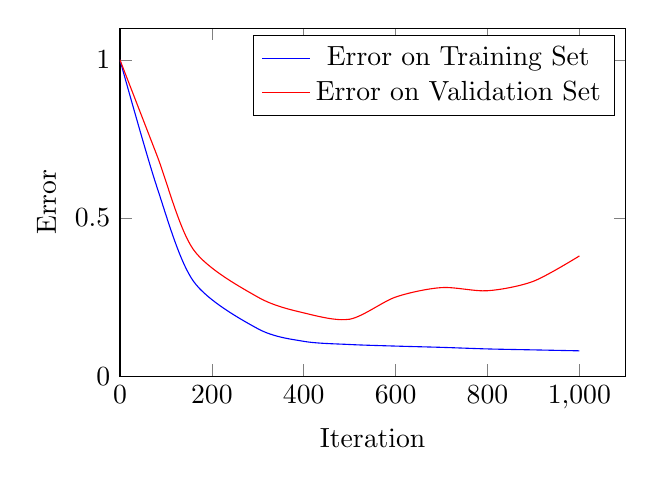
\begin{tikzpicture}
		\begin{axis}[height=6cm,width=8cm,ylabel=Error,xlabel=Iteration,xmin=0,ymin=0]
			\addplot[blue,smooth] coordinates{(0,1)(80,0.6)(160,0.3)(300,0.15)(400,0.11)(500,0.1)(600,0.095)(700,0.091)(800,0.086)(900,0.083)(1000,0.08)};
			\addlegendentry{Error on Training Set}
			\addplot[red,smooth] coordinates{(0,1)(80,0.7)(160,0.4)(300,0.25)(400,0.2)(500,0.18)(600,0.25)(700,0.28)(800,0.27)(900,0.3)(1000,0.38)};
			\addlegendentry{Error on Validation Set}
		\end{axis}
	\end{tikzpicture}
    	\caption[Early stopping based on a validation set.]{The error on the validation set (red) is usually getting larger when the network begins to overfit the training set. Thus, although the error on the training set (blue) is decreasing monotonically, we may want to stop training early to avoid overfitting.}
    	\label{fig:early-stopping}
\end{SCfigure}

\subsubsection{L2-Regularization}

Large weights result in an approximation with poor generalization capabilities. Therefore we try to penalize large weights such that we have \cite[p.~338-343]{Bishop:1995}:
\begin{align}
\hat{E}(w) = E(w) + \eta w^T w.
\end{align}
This regulizer is also referred to as weight decay. For understanding why this regulizer is called weight decay, we consider the derivative of the error function $\hat{E}$ which is given by
\begin{align}
\nabla \hat{E} = \nabla E + \eta w\onedot
\end{align}
Neglecting $\nabla E$ and considering gradient descent learning the change in $w$ with respect to the iteration step $t$ can be described as
\begin{align}
\label{eq:weight-decay-derivative}
\frac{\partial}{\partial t} w[t] = - \gamma \eta w[t]\onedot
\end{align}
Equation \eqref{eq:weight-decay-derivative} has the solution $w[t] = w[0] e^{- \gamma \eta t}$ such that the weights tend exponentially to zero -- giving the method its name \cite[p.~338-340]{Bishop:1995}. While weight decay represents L2-regularization we could also consider L1-regularization.

\subsubsection{Early Stopping}

Early stopping describes the approach to stop training before gradient descent has finished. The error on the training set is usually monotonically decreasing with respect to the iteration number. For unseen data the error is usually much higher and not monotonically decreasing. It tends to get larger when we reach a state of over-fitting. Therefore, it seems reasonable to stop training at a point where the error on the validation set reaches a minimum \cite[p.~343-345]{Bishop:1995}. This is illustrated in figure \ref{fig:early-stopping}.

% \subsubsection{Training invariances}

% Additionally to the training data we often have prior knowledge about desired mapping of the neural network. This includes invariances -- the output should be unchanged if the data istransformed in some specified way.